\documentclass[10pt,a4paper]{article}
\setlength{\parskip}{\baselineskip}%
% \setlength{\parindent}{0pt}%
\usepackage{indentfirst}
\usepackage{url}
% \usepackage{minted}
% \usemintedstyle{manni}
\usepackage{listings}

% \usepackage{siunitx}
% \sisetup{table-number-alignment=center, exponent-product=\cdot}




\usepackage{xcolor} % for setting colors
\usepackage[most]{tcolorbox}



\definecolor{light-gray}{gray}{0.95}
\newcommand{\code}[1]{\colorbox{light-gray}{\lstinline{#1}}}


\lstset{%
  language=python,
  commentstyle=\bfseries,
  escapeinside={(*@}{@*)}
}

\definecolor{codegreen}{rgb}{0,0.6,0}
\definecolor{codegray}{rgb}{0.5,0.5,0.5}
\definecolor{codecyan}{rgb}{0.2, 0.4, 0.7}
\definecolor{backcolour}{rgb}{0.96,0.96,0.98}
\definecolor{dark}{rgb}{0.3,0.3,0.3}


\lstdefinestyle{mystyle}{
    backgroundcolor=\color{backcolour},   
    rulecolor=\color{backcolour},
    commentstyle=\color{codegreen},
    framexleftmargin=1pt,
    numbers=left,
    xleftmargin=2em,
    frame=single,
    framexleftmargin=1.5em,
     framextopmargin=1mm,
     framexbottommargin=1mm,
    keywordstyle=\color{codecyan},
    identifierstyle = \color[rgb]{0.0,0.4,0.4},
    numberstyle=\color{codegray}\ttfamily,
    stringstyle=\color{codecyan},
    basicstyle=\ttfamily\color{dark},
    breakatwhitespace=false,         
    breaklines=true,                 
    captionpos=b,                    
    keepspaces=true,           
    numbersep=5pt,                  
    showspaces=false,                
    showstringspaces=false,
    showtabs=false,                  
    tabsize=2,
}
\lstset{style=mystyle}
% \usepackage{pythonhighlight}
\usepackage[utf8]{inputenc}
\usepackage[portuguese]{babel}
\usepackage[T1]{fontenc}
\usepackage{amsmath}
\usepackage{graphicx}

\usepackage{amsfonts}
\usepackage{amssymb}
\graphicspath{ {./plots/} }
\author{João Viktor Souza Almeida}
\title{Análise de diferentes algoritmos de ordenação}



\begin{document}
\begin{titlepage} %iniciando a "capa"
    \begin{center} %centralizar o texto abaixo
    {\large Universidade de São Paulo}\\[0.2cm] %0,2cm é a distância entre o texto dessa linha e o texto da próxima
    {\large Instituto de Matemática e Estatística}\\[0.2cm] % o comando \\ "manda" o texto ir para próxima linha
    {\large Departamento de Ciência da Computação}\\[0.2cm]
    {\large Bacharelado em Ciência da Computação}\\[0.2cm]
    {\large MAC110 - Introdução à Computação}\\[5.1cm]
    {\bf \huge Análise de diferentes algoritmos de ordenação}\\[5.1cm] 
    \end{center} %término do comando centralizar
    {\large Aluno: João Viktor Souza Almeida}\\[0.7cm] % o comando \large deixa o texto grande
    {\large NUSP: 15521614}\\[0.7cm] % o comando \large deixa o texto grande
    {\large Turma: MAC0110-145-2024}\\[0.7cm] % o comando \large deixa o texto grande
    {\large Professor: Roberto Hirata Junior}\\[5.1cm]
    \end{titlepage} %término da "capa"

\subsection*{Resumo}
O relatório a seguir visa dissertar acerca algoritmos de ordenação clássicos, tais como bolha, contagem, inserção e seleção, bem como investigar exemplos, apresentar a implementação em Python e elucidar como o algoritmo se comporta ao ordenar uma lista.
Além disso, é verificado como a eficiência dos algoritmos variam dadas diferentes condições iniciais, tais como porcentagem de ordenação e composição da lista a ser ordenada. 
Por fim, foram implementados os algoritmos na linguagem C a fim de analisar os seus comportamentos em uma linguagem compilada, em contraste com a linguagem utilizada, Python, que é interpretada.
\

\subsection*{Abstract}
The following report seeks to dissertate the classic ordering algorithms, such as bubble, counting, insertion, and selection, as well as investigate examples, present Python's implementation, and elucidate how each algorithm comports when ordering a list.
In addition, it is verified how the efficiency varies given different initial conditions, like the ordination percentage and the list composition.
Finally, the algorithms were implemented in C to analyze how they comport in a compiled language, contrasting with Python, an interpreted language.

\section*{Metodologia}
Na criação do relatório, os testes dos algoritmos foram realizados utilizando a linguagem de programação Python, com a versão 3.10.11, no sistema operacional Windows.
Além disso, os arquivos em C foram compilados utilizando o GCC na versão 13.1.0.

Durante a execução dos algoritmos, foi utilizada uma máquina com as seguintes configurações:

\begin{itemize}
\item    Processador (CPU): Ryzen 5 3350G 
\item Memória (RAM): 16GB DDR4 @ 3200MHz
\item Armazenamento: 256GB SSD
\item Placa de Vídeo (GPU): Radeon Vega 11
\item Sistema Operacional: Windows 11 Pro
\end{itemize}
% TODO revisar o código
Adicionalmente, a fim de minimizar possíveis interferências nos resultados dos testes, os códigos foram executados com o mínimo de programas em segundo plano. 
Para computar a média de execução, foi criada uma função na qual que retornava a média e o desvio padrão das 10 itinerações do mesmo algoritmos.
Além disso, foram ignoradas possíveis margens de erros da função que embaralha as listas. Contudo, essa margem de erro torna-se desprezível devido ao tamanho das listas utilizadas.

Por fim, na implementação dos códigos na linguagem C, foi importada a biblioteca externa \code{stdbool.h} a fim de criar variáveis booleanas. Além disso, para possibilitar a importação das funções para o arquivo em Python, foi executado, no terminal, o comando \code{gcc -shared -fPIC -o libsortings.so main.c}, cuja função foi transformar as funções em uma biblioteca, possibilitando a invocação destes no Python.

\noindent\textbf{Palavras-chave:} insertion, bubble, counting, selection, algoritmos, ordenação, análise;

\subsection*{Testes}
    Para a realização do relatório, foram realizados dois testes. 
    O primeiro focou em observar os impactos causados pelo tamanho da lista a ser ordenada, ou seja, como o desvio padrão e a média mudam ao aumentar ou diminuir o tamanho da lista a ser ordenada por cada algoritmo. 
    Para isso, foi criada uma malha de repetição e computados as médias e os desvios-padrões de cada algoritmo com listas de tamanhos 1000, 5000, 10000, 50000 e 100000.
    
    O segundo, por outro lado, visou elucidar acerca das mudanças causadas pela taxa de ordenação de uma lista.
    Para isso, foi estabelecida uma segunda malha de repetição, na qual também foram computados as médias e os desvios-padrões de cada algoritmo, mas com uma lista de 100000 elementos e com porcentagens de ordenação de 1\%, 3\%, 5\%, 10\% e 50\%.
    

    Para computar a média, foi criada uma função cujos parâmetros são uma lista e o tamanho desta, respectivamente. O desvio padrão, sob o mesmo ponto de vista, foi calculado por meio de uma função que recebe os mesmos parâmetros que a função outrora citada.
    


\newpage
\tableofcontents
\section{Algoritmo de seleção}
O algoritmo de seleção é um algoritmo de ordenação no qual, a cada itineração, o menor elemento da lista é garantido estar na posição correta. Dessa forma, na primeira itineração, assegura-se que o menor elemento ficará na primeira posição da lista, na segunda itineração, o segundo elemento, e assim por diante. 
Uma observação pertinente é que a quantidade de comparações a ser feita independe da porcentagem de ordenação da lista.

\subsection{Exemplo}
Seja M uma lista \code{[4,3,2,1,0]}. Na primeira passagem, o algoritmo detectará o menor elemento da lista e, logo após, irá permutá-lo com o primeiro elemento da lista, ou seja, o elemento 4 e 0 serão trocados de lugar. Na segunda passagem, começando pelo segundo elemento, a segunda malha de repetição irá detectar o segundo menor elemento e, similarmente, irá permutá-lo com o segundo elemento da lista. Nas próximas execuções, a forma é análoga.

Na n-ésima passagem, onde $n$ é o tamanho da lista, todos os elementos estarão em ordem crescente e, portanto, ordenados.

Assim, seguem as impressões da lista a cada modificação.

\begin{lstlisting}
[4, 3, 2, 1, 0]
[0, 3, 2, 1, 4]
[0, 1, 2, 3, 4]
[0, 1, 2, 3, 4]
[0, 1, 2, 3, 4]
[0, 1, 2, 3, 4]
\end{lstlisting}

Percebe-se que, mesmo a lista já estando ordenada, o algoritmo continuará realizando os comandos, ou seja, o número de passagens a ser feita não é mudado devido às condições iniciais de ordenação.

\newpage
\subsection{Implementação}
A seguir, segue a implementação do código em Python.

\begin{lstlisting}
def selection(V, n):
    for i in range(0, n):
        smallest_num_index = i
        for j in range(i, n):
            if V[j] < V[smallest_num_index]:
                smallest_num_index = j
        V[i], V[smallest_num_index] = V[smallest_num_index], V[i]

\end{lstlisting}
De fato, pelo código percebe-se que não há nenhum mecanismo implementado a fim de detectar a ordenação total da lista e, consequentemente pará-lo.

\subsection{Quantidade de comparações}
Nesta subseção, irá ser debatida a quantidade de comparações feitas pelo algoritmo em questão. Como a quantidade de comparações é independe da ordenação neste algoritmo, será simples de analisá-la; nos outros algoritmos, contudo, a análise é mais complexa devido à oscilação na quantidade de comparações.

Suponha-se que o algoritmo recebeu uma lista com $n$ elementos. Assim, como não há um dispositivo que pare o código antes, tem-se que a primeira malha de repetição será executada $n-i$ vezes, em que o índice inicial $i=0$. Na segunda execução, quando o índice $i=1$, serão realizadas $n-1$ comparações e assim por diante. Por consequência, em cada uma dessas execuções, a segunda malha de repetição (a qual está na primeira) será executada $n-i$ vezes, isto é, o código será executado $n+(n-1)+(n-2)+\cdots+(1) = \sum_{i=1}^n i = \frac{n(n+1)}{2}$ vezes.

Notavelmente, não há variações na quantidade de comparações e, consequentemente, a forma como o código será executado é a mesma independentente do estado inicial da lista.
\section{Algoritmo de bolha}
O algoritmo de bolha é um algoritmo cuja complexidade é, assim como o anterior, quadrática. Sua principal característica é que, na n-ésima passagem pela lista, o algoritmo assegura estarem ordenados os n últimos elementos da lista.

\textbf{Exemplo}: Seja $M$ uma lista [4,3,2,1,0].
Na primeira passagem, o maior valor da lista (4) estará em seu lugar correto, ou seja, M será [3,2,1,0,4]. Na segunda passagem, o segundo maior elemento também estará posicionado em sua posição correta; assim, M será [2,1,0,3,4].

O algoritmo continuará realizando "isto" até que, na 5º passagem, (pois a lista possui 5 elementos), a lista estará totalmente ordenada.

\begin{lstlisting}
def bubble(V, n):
    lim = n - 1
    while lim >= 0:
        isIncreasing = True
        for j in range(lim):
            if V[j] > V[j + 1]:
                isIncreasing = False
                V[j], V[j + 1] = V[j + 1], V[j]
        if(isIncreasing==True): 
                break
        lim -= 1
\end{lstlisting}

De acordo com o código, constata-se que, ao contrário do algoritmo anterior, este não realizará todas as etapas caso a lista já esteja ordenada, pois a variável $isIncreasing$ indica se a lista já se encontra ou não ordenada.
\section{Algoritmo de inserção}
O algoritmo de inserção possui, como principal característica, a asseguração de que, a cada itineração $n$, os n-ésimos primeiros elementos estarão ordenados. Além disso, assim como o de bolha, este varia com a porcentagem de ordenação da lista recebida, ou seja, caso a lista já esteja ordenada, será detectado logo na primeira passagem e, assim, não haverá nada a ser feito. 


\subsection{Exemplo}
Seja, para fins de exemplificação, $V$ a lista $[4,3,2,1,0]$.  

O algoritmo em questão funcionará da seguinte forma: a lista começa dada como ordenada até que se ache um $j$ tal que $V[j]>V[j+1]$, onde $j$ é um inteiro maior ou igual a zero e menor que o tamanho da lista menos um. 
Caso isso ocorra, o algoritmo trocará os dois valores e comparará, da mesma forma, $V[j-1]$ e $V[j]$. Quando o valor da antiga posição $j$ for menor do que a posição sucessora, garante-se, então, que a lista está ordenada de 0 até $j+1$. Contudo, caso não exista um $j$, então o algoritmo indica que a lista já está ordenada e, assim, evita mais comparações.
\\

Logo, tomando a lista $M$, caso esta fosse impressa a cada modificação, os resultados seriam:
\begin{lstlisting}
[4, 3, 2, 1, 0]
[3, 4, 2, 1, 0]
[3, 2, 4, 1, 0]
[2, 3, 4, 1, 0]
[2, 3, 1, 4, 0]
[2, 1, 3, 4, 0]
[1, 2, 3, 4, 0]
[1, 2, 3, 0, 4]
[1, 2, 0, 3, 4]
[1, 0, 2, 3, 4]
[0, 1, 2, 3, 4]
\end{lstlisting}

Visivelmente, observa-se que, sempre que é encontrado um elemento $e$ menor que o anterior, ambos são trocados e, em seguida, o algoritmo começa a verificar e mover $e$ para trás até o elemento em questão fique em sua posição correta.
\newpage

\subsection{Implementação}
Como pode-se perceber, quando é encontrado um elemento $j$ menor do que o anterior, este é "levado" para trás até que esteja na posição correta

\begin{lstlisting}
def insertion(V, n):
last_index = 0
for i in range(last_index,n - 1):
    if V[i] > V[i + 1]:
        j = i
        while V[j] > V[j + 1]:
            V[j + 1], V[j] = V[j], V[j + 1]
            if j <= 0:
                break
            j -= 1
\end{lstlisting}

\subsection{Quantidade de comparações}
Tendo em vista que as comparações realizadas depende da lista, os casos serão analisados. 

Caso a lista com $n$ elementos esteja em ordem, o algoritmo detectará na primeira itineração devido à permanência do valor verdadeiro da variável \code{isIncreasing}, ou seja, serão realizadas $n$ comparações.

Por outro lado, na hipótese da lista está totalmente desordenada, haverá $n(n+1)\over 2$. A prova é análoga à do bolha.

Finalmente, nos outros casos, a análise é, assim como no algoritmo anterior, compléxa. Contudo, em cenários nos quais a lista não se enquadra nos casos supracitados, o algoritmo possui um comportamento quadrático.
%TODO citar fonte
\section{Algoritmo de contagem}
Diferentemente dos algoritmos outrora discutidos, o contagem possui uma complexidade linear, isto é, o tempo levado para ordenar cresce proporcionalmente com o tamanho da lista recebida. 

Em relação ao uso de memória, contudo, há uma grande desvantagem no algoritmo: devido ao uso de uma lista auxiliar, esta possuirá $\max({lista})-\min({lista}) $ elementos; ou seja, caso o maior elemento seja 5000 e o menor 1000, a lista auxiliar possuirá de 4000 elementos.

Dessa forma, o algoritmo possui um melhor proveito se utilizado para listas com pouca variação de tamanho entre os seus elementos.

\subsection{Exemplo}
Seja $M$ a lista $[4,2,3,1,4,2,2,0]$. Como a diferença entre o maior e o menor é elemento é 4, a lista auxiliar $Aux$ será de tamanho 4.
Assim, a lista auxiliar $Aux$ será da seguinte forma (assumindo que o primeiro elemento é $Aux[0]$): o primeiro elemento terá o valor igual à quantidade de zeros na lista original, que é 1, o segundo elemento também será 1 por motivo análogo, e o terceiro elemento de $Aux$, por outro lado, receberá o valor 3, uma vez que há três elementos 2 na lista original. Essa lógica prevalecerá até último elemento.
Assim, de início, a lista $Aux$ será [1,1,3,1,2].

Em seguida, começará a modificação da lista original: serão adicionados à lista original $n$ vezes o elemento referente ao índice da lista auxiliar, ou seja, como $Aux[0]$ é igual a 1, será adicionado um zero a $M$ (adicionando da esquerda para a direita e um ao lado do outro). Em $Aux[2]$, por exemplo, o elemento é 3 e, assim, será adicionado o elemento 2 três vezes seguidas à lista $M$.

Seguem os valores de \code{Aux} a cada modificação:
\begin{lstlisting}
[0, 0, 0, 0, 0]
[1, 0, 0, 0, 0]
[1, 1, 0, 0, 0]
[1, 1, 3, 0, 0]
[1, 1, 3, 1, 0]
[1, 1, 3, 1, 2]
\end{lstlisting}
\newpage
Para fins elucidativos, serão substituídos por "0" os elementos já existentes em $M$ a fim de mostrar os valores adicionados posteriormente, ou seja, supor-se-á que a lista $M$ teve todos os seus valores trocados para 0.
\begin{lstlisting}
[0, 0, 0, 0, 0, 0, 0, 0]
[0, 0, 0, 0, 0, 0, 0, 0]
[0, 1, 0, 0, 0, 0, 0, 0]
[0, 1, 2, 0, 0, 0, 0, 0]
[0, 1, 2, 2, 0, 0, 0, 0]
[0, 1, 2, 2, 2, 0, 0, 0]
[0, 1, 2, 2, 2, 3, 0, 0]
[0, 1, 2, 2, 2, 3, 4, 0]
[0, 1, 2, 2, 2, 3, 4, 4] 
\end{lstlisting}

Percebe-se, portanto, que a lista foi ordenada realizando-se nenhuma comparação.

\subsection{Implementação}
Segue a implementação do algoritmo em questão em Python:

\begin{lstlisting}
def counting(V, n):
    max_element = max(V)
    hist_list = [0 for _ in range(max_element + 1)]
    for i in range(max_element + 1):
        hist_list[i] = count_element_in_array(i, V)
    index = 0
    for i in range(max_element + 1):
        for _ in range(hist_list[i]):
            V[index] = i
            index += 1
\end{lstlisting}
Como se pode perceber, o algoritmo de contagem, assim como os outros, possui duas malhas de repetição. Contudo, em vez de as malhas estarem aninhada, uma ocorre após a outra.
Apesar disso, uma singularidade desse algoritmo é que, ao contrário dos citados, a quantidade de itinerações na primeira malha de repetição depende do tamanho do maior elemento (pensando apenas na implementação com números positivos), tornando-o eficaz para listas grandes e com elementos menores.

\subsection{Quantidade de comparações}
Diferentemente de todos os algoritmos outrora citados, este não realiza qualquer comparação.


\section{Resultados}
Nesta seção, será debatido acerca dos resultados obtivos por meio dos dois testes realizados. O primeiro visou analisar o tempo médio de cada algoritmo, bem como a sua variância. No segundo teste, por outro lado, buscou-se avaliar o comportamento dos algoritmos bolha e inserção quando submetidos a listas com diferentes taxas de ordenação, sendo elas 1\% , 3\%, 5\%, 10\% e, por fim, 50\%. 

Logo abaixo, têm-se os resultados em gráficos.

\subsection{Variação na quantidade de elementos}
Como outrora comentado, os resultados comprovam o comportamento quadrático do bolha, seleção e inserção. 

Contudo, é necessário destacar que, caso houvesse uma maior variância nos números da lista a ser ordenada, isto é, caso a diferença entre o maior e o menor valor fosse um valor muito grande, o algoritmo de contagem apresentaria um resultado ruim, podendo ultrapassar o bolha, por exemplo.
\begin{figure}[h]
    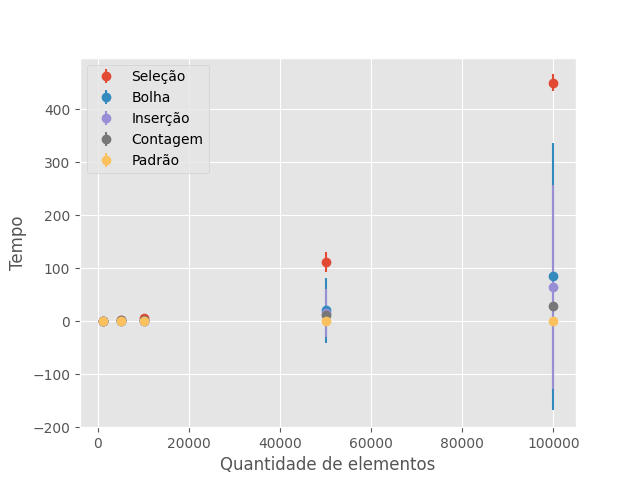
\includegraphics[width=8cm]{sizes.png}
    \caption{Gráfico elucidando o comportamento de cada algoritmo em tópico. No eixo x, há a quantidade de elementos; no y, o tempo médio gasto, em segundos, por cada algoritmo}
    \end{figure}

    \subsection{Ordenação prévia}
    \begin{figure}[h]
        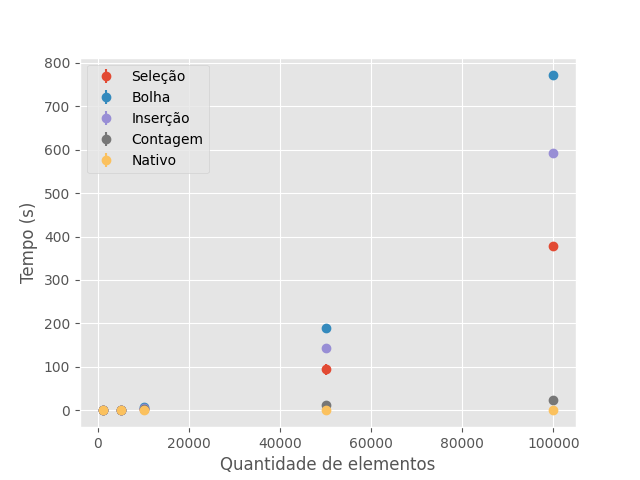
\includegraphics[width=8cm]{result_1717775798.8843806.png}
        \caption{Gráfico ilustrando o tempo médio 'gasto' dos algoritmos bolha e inserção em relação à taxa de ordenação inicial dos vetores.}
    \end{figure}

Como  previamente comentado, o algoritmo de bolha e o de inserção variam de acordo com a taxa de ordenação. Assim, em caso de ordenação inicial total, ambos os algoritmos adquirem um comportamento linear, uma vez que serão feitas $n$ comparações até que o algoritmo detecte que a lista já se encontra ordenada e, consequentemente, parará.

\section{Implementação em C}
Nesta seção, implementaram-se, na linguagem C, os algoritmos em tópico a fim de analisar os impactos no desempenho quando executado um algoritmo em uma linguagem compilada, tal como o C.
Após visto o comportamento dos algoritmos em Python, uma linguagem interpretada, percebe-se que, mesmo para vetores pequenos, o tempo gasto para ordená-los é significativo.

Quando implementados utilizando a linguagem C, contudo, nota-se uma considerável redução na duração dos testes, uma vez que, em razão do C ser uma linguagem compilada, as malhas de repetição tendem a ser mais eficientes.
Ademais, ao utilizar a linguagem C, há um maior controle na forma como o código será executado, devido ao C ser uma linguagem com um nível mais baixo e tipada, em outras palavras, há uma possibilidade de otimizar o código de maneira mais eficaz.


Dessa forma, serão analisados os desempenhos de alguns dos algoritmos já implementados em Python, mas, desta vez, estes serão escritos na linguagem C.
A fim de realizar o testes, os algoritmos foram implementados na linguagem C, utilizando, como referência, os códigos já escritos em Python. Sendo assim, tendo em vista que os códigos utilizandos em C não foram otimizados e nem modificados de forma a deixá-los mais lentos, ter-se-á uma comparação equânime.
Além disso, as funções foram invocadas no Python visando criar os gráficos dos resultados.

Por fim, é necessário ressaltar que foram realizados somentes testes visando analisar o comportamento dos algoritmos em C quando estes são submetidos a sequências com tamanhos variáveis, ou seja, o segundo teste não será executado, pois será obtido resultados similares ao anterior.

\newpage
\subsection{Resultados}
A seguir, serão analisados os resultados encontrados, assim como no primeiro teste, realizando a execução dos algoritmos implementados em C e, para fins comparativos, do algoritmo contagem cuja realização foi feita na linguagem principal.
\begin{figure}[h]
    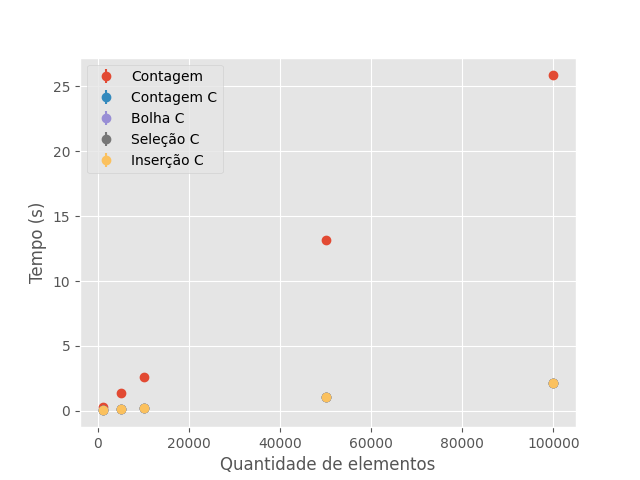
\includegraphics[width=8cm]{c sizes.png}
    \caption{Gráfico ilustrando o tempo médio de execução dos algoritmos implementados em C comparado ao do contagem, implementado em Python.}
\end{figure}
\begin{table}[h]
    \centering
    \begin{tabular}{llllll}
        \textbf{Tamanho} & \textbf{Contagem Py} & \textbf{Contagem} & \textbf{Bolha} & \textbf{Seleção} & \textbf{Inserção} \\
        1000 & 0.2798 & 0.0221 & 0.0222 & 0.0219 & 0.0220 \\
        5000 & 1.3991 & 0.1099 & 0.1088 & 0.1091 & 0.1064 \\
        10000 & 2.5873 & 0.2151 & 0.2136 & 0.2151 & 0.2147 \\
        50000 & 13.1278 & 1.0672 & 1.0653 & 1.0638 & 1.0609 \\
        100000 & 25.9120 & 2.1320 & 2.1423 & 2.1244 & 2.1281 \\
    \end{tabular}
    \caption{Tempos de execução dos algoritmos de ordenação (em segundos) para diferentes tamanhos de lista}
    \label{tab:tempos_ordenacao}
\end{table}

Abaixo, encontram-se os desvios-padrões de cada algoritmo com os respectivos tamanhos das listas ordenadas.
\begin{table}[h]
    \centering
    \begin{tabular}{llllll}
        \textbf{Tamanho} & \textbf{Contagem Py} & \textbf{Contagem} & \textbf{Bolha} & \textbf{Seleção} & \textbf{Inserção} \\

        1000 & 0.001368 & 0.000001 & 0.000002 & 0.0000001 & 0.0000004 \\
        5000 & 0.041076 & 0.000023 & 0.000003 & 0.000002 & 0.000003 \\
        10000 & 0.000821 & 0.000006 & 0.000007 & 0.000017 & 0.000010 \\
        50000 & 0.068934 & 0.000065 & 0.000035 & 0.000022 & 0.000053 \\
        100000 & 0.019201 & 0.000073 & 0.002216 & 0.000139 & 0.000056 \\
    \end{tabular}
    \caption{Desvios padrão dos tempos de execução dos algoritmos de ordenação (em segundos) para diferentes tamanhos de lista}
    \label{tab:desvios_ordenacao}
\end{table}

%TODO melhorar este texto
De início, nota-se que o comportamento dos algoritmos não é modificado, isto é, permaneceram inalteradas, quando implementados em C, características como o uma maior oscilação (maior desvio-padrão) no tempo dos algoritmos que variavam dependendo da taxa de ordenação inicial.
Assim, o comportamento esperado dos algoritmos ainda é visível, independente da linguagem utilizada na implementação.


Perceptivelmente, o ganho de desempenho dos algoritmos implementados em C mostrou-se singificativo; mesmo os mais lentos quando implementados em Python, como o bolha, obtiveram uma performance superior ao contagem da linguagem inicial.
Por outro lado, não houve uma mudança perceptível nos desvios-padrões de cada algoritmo, em outras palavras, a oscilação no tempo necessário em cada algoritmo permaneceu semelhante na implementação em ambas as linguagens.


De fato, o contagem implementado em Python mostrou-se, aproximadamente, 12 vezes mais lento que a sua versão em C quando executado utilizando listas com 100000 elementos. Em listas com tamanhos menores, essa diferença manteu-se quase constante, oscilando entre 12 e 13 vezes mais demorado, ou seja, não há uma variação significante no desempenho em relação à grandeza do vetor. Dessa maneira, é notável que a implementação em C mostrou-se mais eficaz, independente do tamanho da lista.


Portanto, visando um ganho de performance, é recomendável a utilização da linguagem C a fim de implementar algoritmos que se beneficiam de malhas de repetições.
Ademais, caso seja necessário o uso do Python para outras tarefas no projeto, as funções em C podem ser chamadas por meio da criação de bibliotecas e, por meio destas, importá-las no Python.
%TODO revistar
\section{Conclusão}
Desta maneira, apesar de deterem diferentes desempenhos dependendo da ordenação do vetor, os algoritmos em questão possuem um baixo proveito com listas muito grandes. Portanto, a fim de ordenar uma lista com maior rapidez, é aconselhável utilizar a função já implementada do Python, conhecida como timsort.

Adicionalmente, o algoritmo de contagem, ainda que o vetor passado tenha poucos elementos, pode ter um tempo de execução muito alto em razão da variação entre os números. Assim, é aconselhável a utilização do algoritmo em pauta apenas com listas com uma exígua variação.

Em outra perspectiva, o bolha foi o algoritmo que apresentou o menor rendimento quando submetido a sequências com diferentes tamanhos; o contagem, por outro lado, garantiu, apesar da faixa de valores maior, o melhor desempenho, principalmente nas listas com mais elementos. Dessa forma, a utilização do bolha é recomendada apenas para fins didáticos.


Por fim, diante das comparações realizadas entre o Python e C, observa-se que, para algoritmos que dependem de malhas de repetição, a segunda linguagem apresenta um desempenho mais satisfatório.

\section{Considerações finais}
A realização deste relatório possibilitou o aprendizado em diversas áreas do conhecimento, especialmente na análise de algoritmos, ao separá-los por casos e verificá-los individualmente.
Além disso, o projeto proporcionou uma ampla experiência na criação de textos acadêmicos e na investigação da eficiência e do comportamento de um algoritmo.
Portanto, o exercício programa permitiu um aprimoramento em competências que serão de extrema importância para futuros projetos.

\newpage
\begin{thebibliography}{3}
    \bibitem{bubblecomplexity}
    Bubble Sort Time Complexity and Algorithm Explained, builtin, 2023. Disponível em: \url{https://builtin.com/data-science/bubble-sort-time-complexity#:~:text=The%20bubble%20sort%20algorithm%27s%20average,complexity%3A%20O(n%C2%B2)}. Acesso em: 08 de jun. de 2024.
    \bibitem{insertioncomplexity}
    Insertion Sort Explained–A Data Scientists Algorithm Guide, 2021. Disponível em: \url{https://developer.nvidia.com/blog/insertion-sort-explained-a-data-scientists-algorithm-guide/#:~:text=The%20worst%2Dcase%20(and%20average,O(n)%20time%20complexity.}. Acesso em: 08 de jun. de 2024.
\end{thebibliography}


\end{document}